% !TEX program = xelatex
\documentclass[a4paper]{article}

\usepackage{blindtext}
\usepackage[T1]{fontenc}
\usepackage{textcomp}
\usepackage{graphicx}

\title{Environments}
\author{naiithink}
\date{}

\setlength{\parindent}{0pt}

\begin{document}
\begin{titlepage}
\maketitle
\thispagestyle{empty}
\tableofcontents
\end{titlepage}

\newpage
\section{Lists}
\begin{flushleft}
\begin{enumerate}
\item You can nest the list
environments to your taste:
\begin{itemize}
\item But it might start to
look silly.
\item[-] With a dash.
\end{itemize}
\item Therefore remember:
\begin{description}
\item[Stupid] things will not
become smart because they are
in a list.
\item[Smart] things, though,
can be presented beautifully
in a list.
\end{description}
\end{enumerate}
\end{flushleft}

\newpage
\section{Alignment}
\begin{flushleft}
\blindtext
\end{flushleft}

\begin{center}
\blindtext
\end{center}

\begin{flushright}
\blindtext
\end{flushright}

\newpage
\section{Quotes}

\subsection{\texttt{quote}, \texttt{quotation}}
\subsubsection*{\texttt{quote}}
A typographical rule of thumb
for the line length is:
\begin{quote}
On average, no line should
be longer than 66 characters.
\end{quote}
This is why \LaTeX{} pages have
such large borders by default
and also why multicolumn print
is used in newspapers.

\subsubsection*{\texttt{quotation}}
The quotation environment is useful for longer quotes
going over several paragraphs, because it indents the first
line of each paragraph.

\subsection{\texttt{verse}}
I know only one English poem by
heart. It is about Humpty Dumpty.
\begin{flushleft}
\begin{verse}
Humpty Dumpty sat on a wall:\\
Humpty Dumpty had a great fall.\\
All the King's horses and all
the King's men\\
Couldn't put Humpty together
again.
\end{verse}
\end{flushleft}

\newpage
\section{Abstract}
\begin{abstract}
\blindtext
\end{abstract}

\newpage
\section{Printing Verbatim}
The verbatim environment and the \texttt{\char92 verb} command may not be used within parameters of other commands.

\subsection{As a Block}
\begin{verbatim}
#include <stdio.h>

int main(void)
{
    printf("hello, world\n");
    return 0;
}
\end{verbatim}

\subsubsection*{The \texttt{*} version}
\begin{verbatim*}
#include <stdio.h>

int main(void)
{
    printf("hello, world\n");
    return 0;
}
\end{verbatim*}

\subsection{Interpolate}
Or within a \verb+paragraph+ eiei.\\
The \verb|+| is just an example of a delimiter character.\\
Use any character except letters, \verb|*| or space. Many \LaTeX{} examples in this booklet are typeset with this command.

\subsubsection*{Also has a \texttt{*} version}
\verb*|like this :-) |

\newpage
\section{Tabulation}
\fbox{\texttt{\textbackslash{}begin\{tabular\}[pos]\{table spec\}}}

\subsection*{\texttt{table spec}}
\begin{tabular}{c @{~~~~} l}
\texttt{l} & column of left-aligned text\\
\texttt{r} & right-aligned text\\
\texttt{c} & centered text\\
\texttt{p\{width\}} & column containing justified text with line breaks\\
\texttt{\textbar} & vertical line
\end{tabular}

\rule{0pt}{2ex}

If the text in a column is too wide for the page, \LaTeX{} won't automatically wrap it.
Using \verb+p{width}+ you can define a special type of column which will wrap-around the text as in a normal paragraph.

\subsection{Simple Table}
\begin{tabular}{|r|l|}
\hline
7C0 & hexadecimal \\
3700 & octal \\ \cline{2-2}
11111000000 & binary \\
\hline \hline
1984 & decimal \\
\hline
\end{tabular}

\subsection*{Wrapping}
\begin{tabular}{|p{4.7cm}|}
\hline
Welcome to Boxy's paragraph.
We sincerely hope you'll
all enjoy the show.\\
\hline
\end{tabular}

\subsection*{Leading Spaces}
\begin{tabular}{l | l}
\hline \\
\begin{tabular}{@{} l @{}}
\hline
no leading space\\
\hline
\end{tabular} &
\begin{tabular}{l}
\hline
leading space left and right\\
\hline
\end{tabular}\\\\
\hline
\end{tabular}

\subsection*{Decimal Point}
\begin{tabular}{c r @{.} l}
Pi expression       &
\multicolumn{2}{c}{Value} \\
\hline
$\pi$               & 3&1416  \\
$\pi^{\pi}$         & 36&46   \\
$(\pi^{\pi})^{\pi}$ & 80662&7 \\
\end{tabular}

\subsection*{Column Labeling}
\begin{tabular}{l | l}
\hline \\
\begin{tabular}{c r @{.} l}
Pi expression       &
\multicolumn{2}{c}{Value} \\
\hline
$\pi$               & 3&1416  \\
$\pi^{\pi}$         & 36&46   \\
$(\pi^{\pi})^{\pi}$ & 80662&7 \\
\end{tabular} &
\begin{tabular}{|c|c|}
\hline
\multicolumn{2}{|c|}{Ene} \\
\hline
Mene & Muh! \\
\hline
\end{tabular}\\
\hline
\end{tabular}

\newpage
\subsection{\texttt{\textbackslash{}arraystretch} and \texttt{\textbackslash{}tabcolsep}}
\begin{tabular}{|l|}
\hline
These lines\\\hline
are tight\\\hline
\end{tabular}
{\renewcommand{\arraystretch}{1.5}
\renewcommand{\tabcolsep}{0.2cm}
\begin{tabular}{|l|}
\hline
less cramped\\\hline
table layout\\\hline
\end{tabular}}

\subsubsection*{Single Row Height}
\begin{tabular}{|c|}
\hline
\rule{1pt}{4ex}Pitprop \ldots\\
\hline
\rule{0pt}{4ex}Strut\\
\hline
\end{tabular}

\newpage
\subsection{Long Tables}
\fbox{to be continued\ldots}
% \begin{longtable}{| l | l |}
% \hline
% \blindtext[5] & \blindtext[5]\\
% \hline
% \end{longtable}

\newpage
\section{Including Graphics and Images}

\subsection{\texttt{graphicx} Package}

\fbox{\texttt{\textbackslash{}includegraphics[key=value]\{filename\}}}

\begin{table}[!ht]
\caption{Key Names}
\begin{tabular}{l|l}
\texttt{width}      &       scale graphic to the specified width        \\
\texttt{height}     &       scale graphic to the specified height       \\
\texttt{angle}      &       rotate graphic counterclockwise             \\
\texttt{scale}      &       scale graphic
\end{tabular}
\end{table}

\newpage
\begin{verbatim}
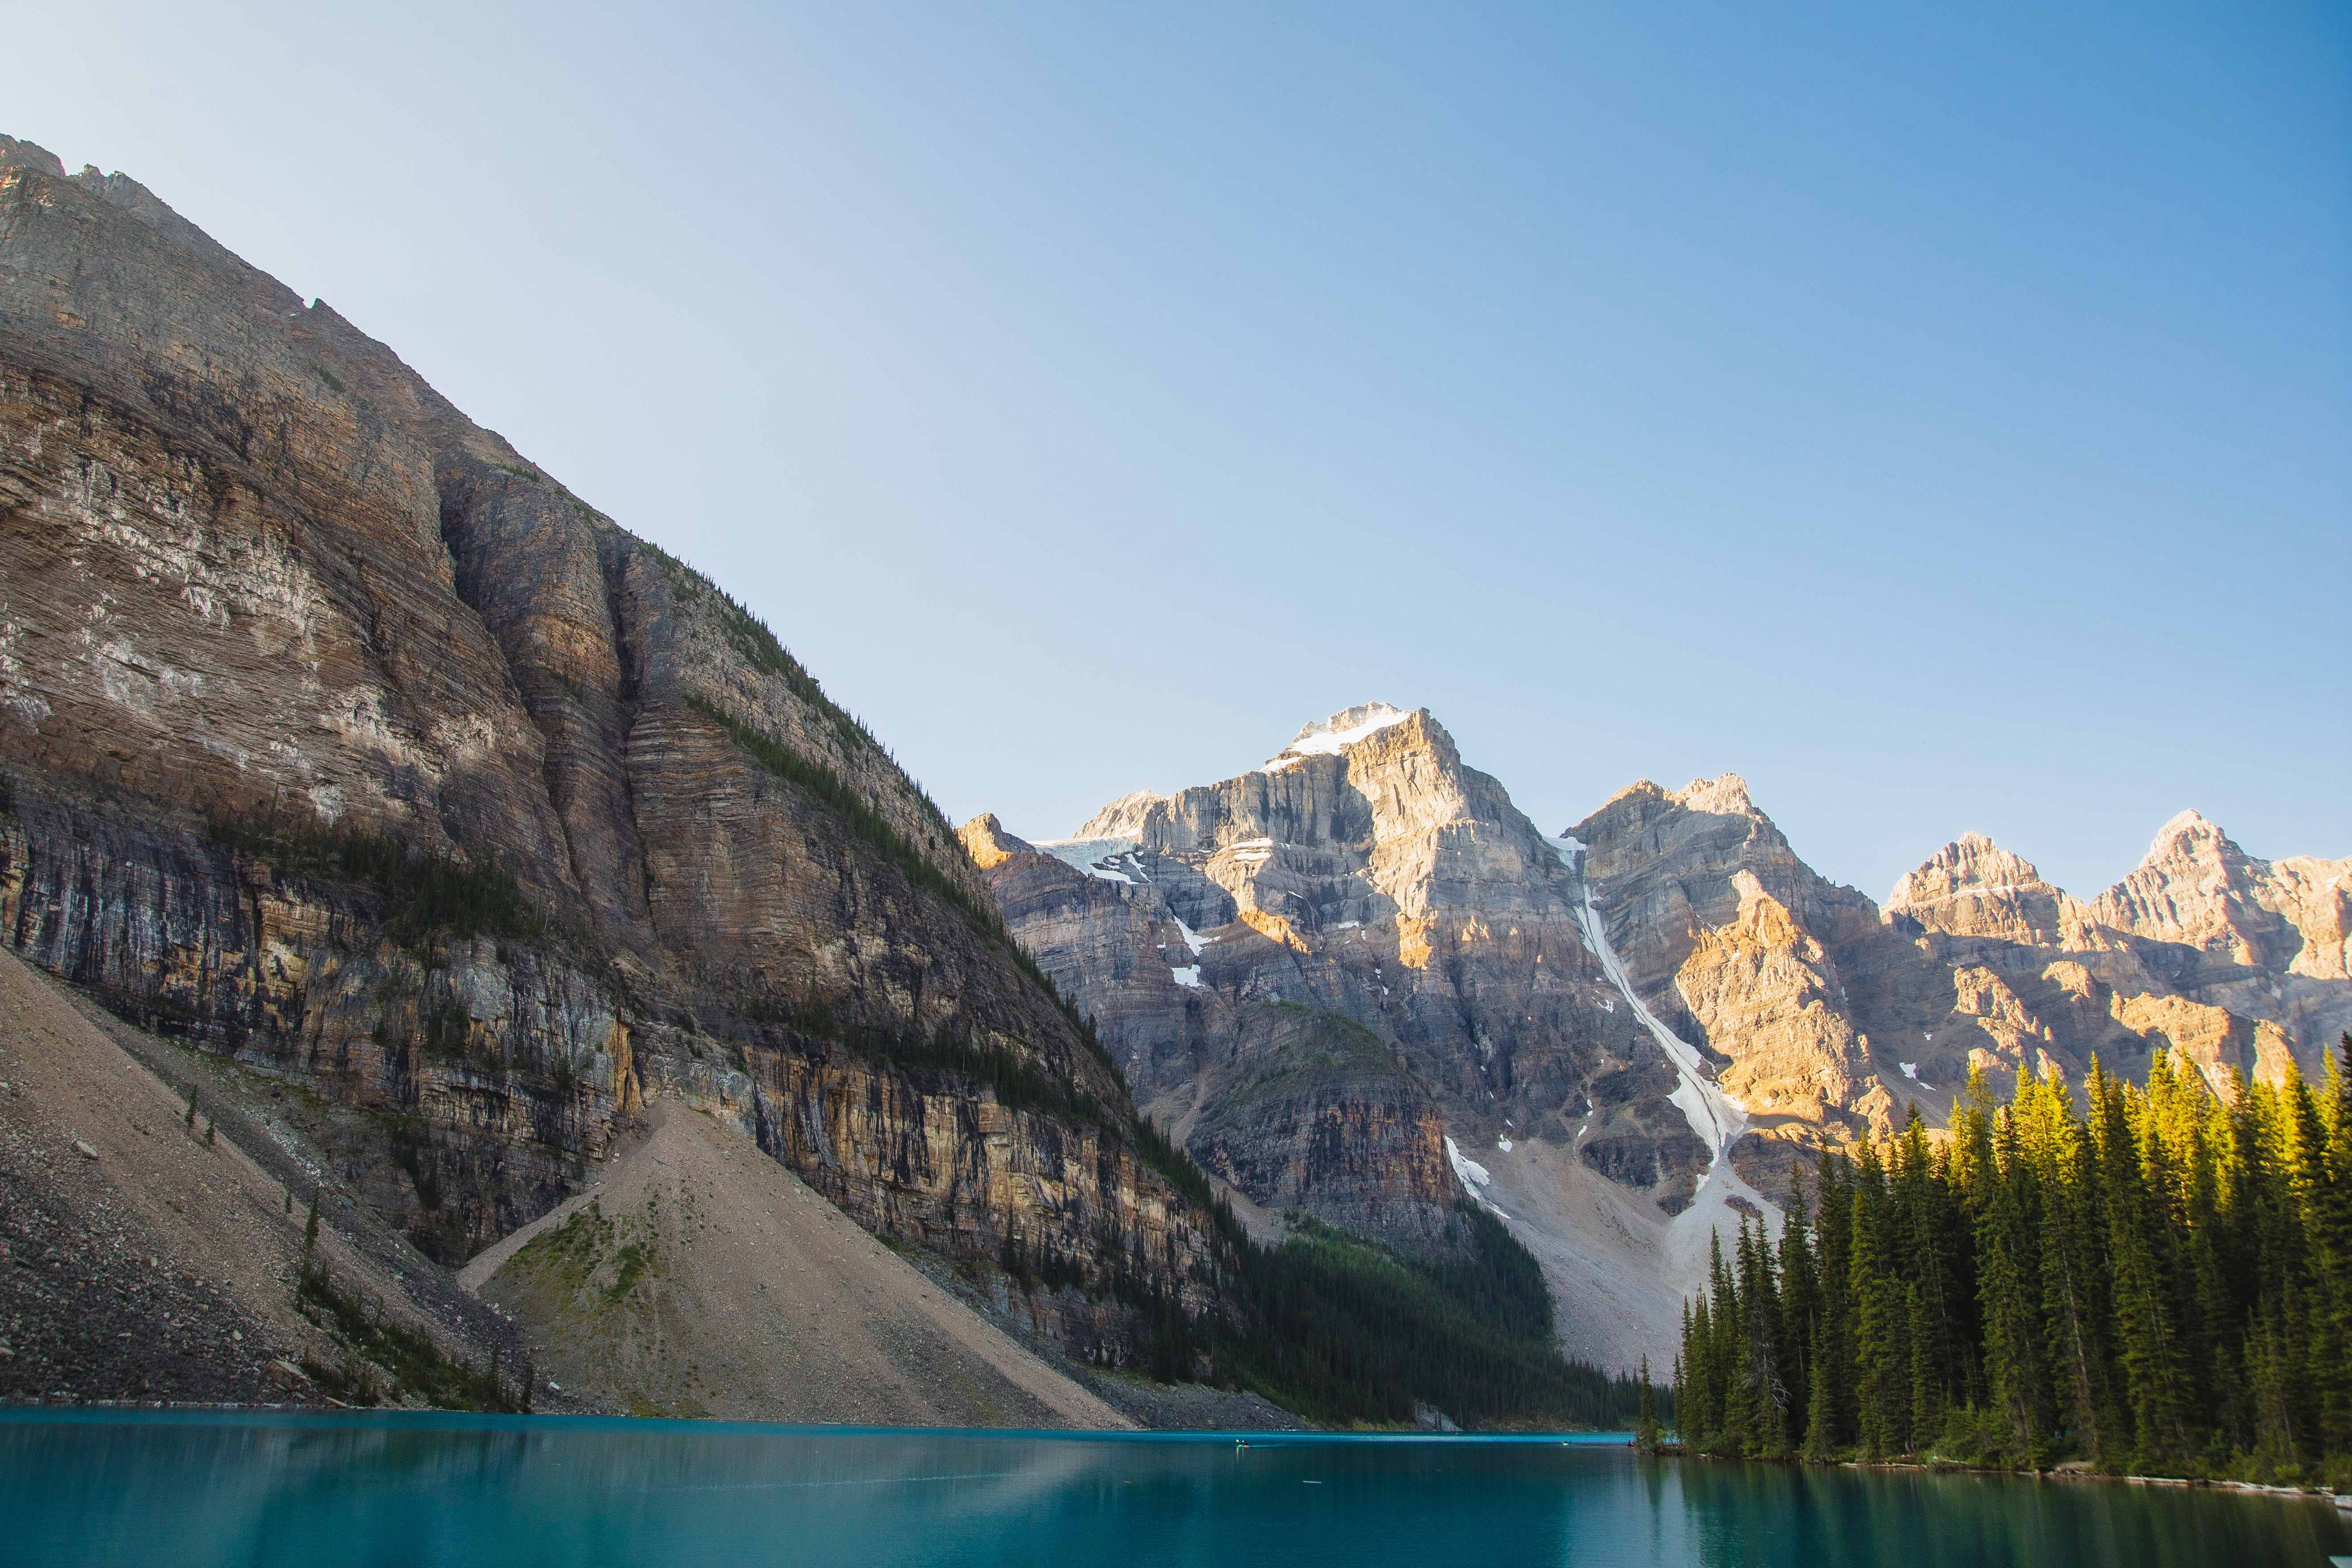
\includegraphics[angle=90,width=\textwidth]{img/mountain.jpg}
\end{verbatim}

\begin{flushleft}
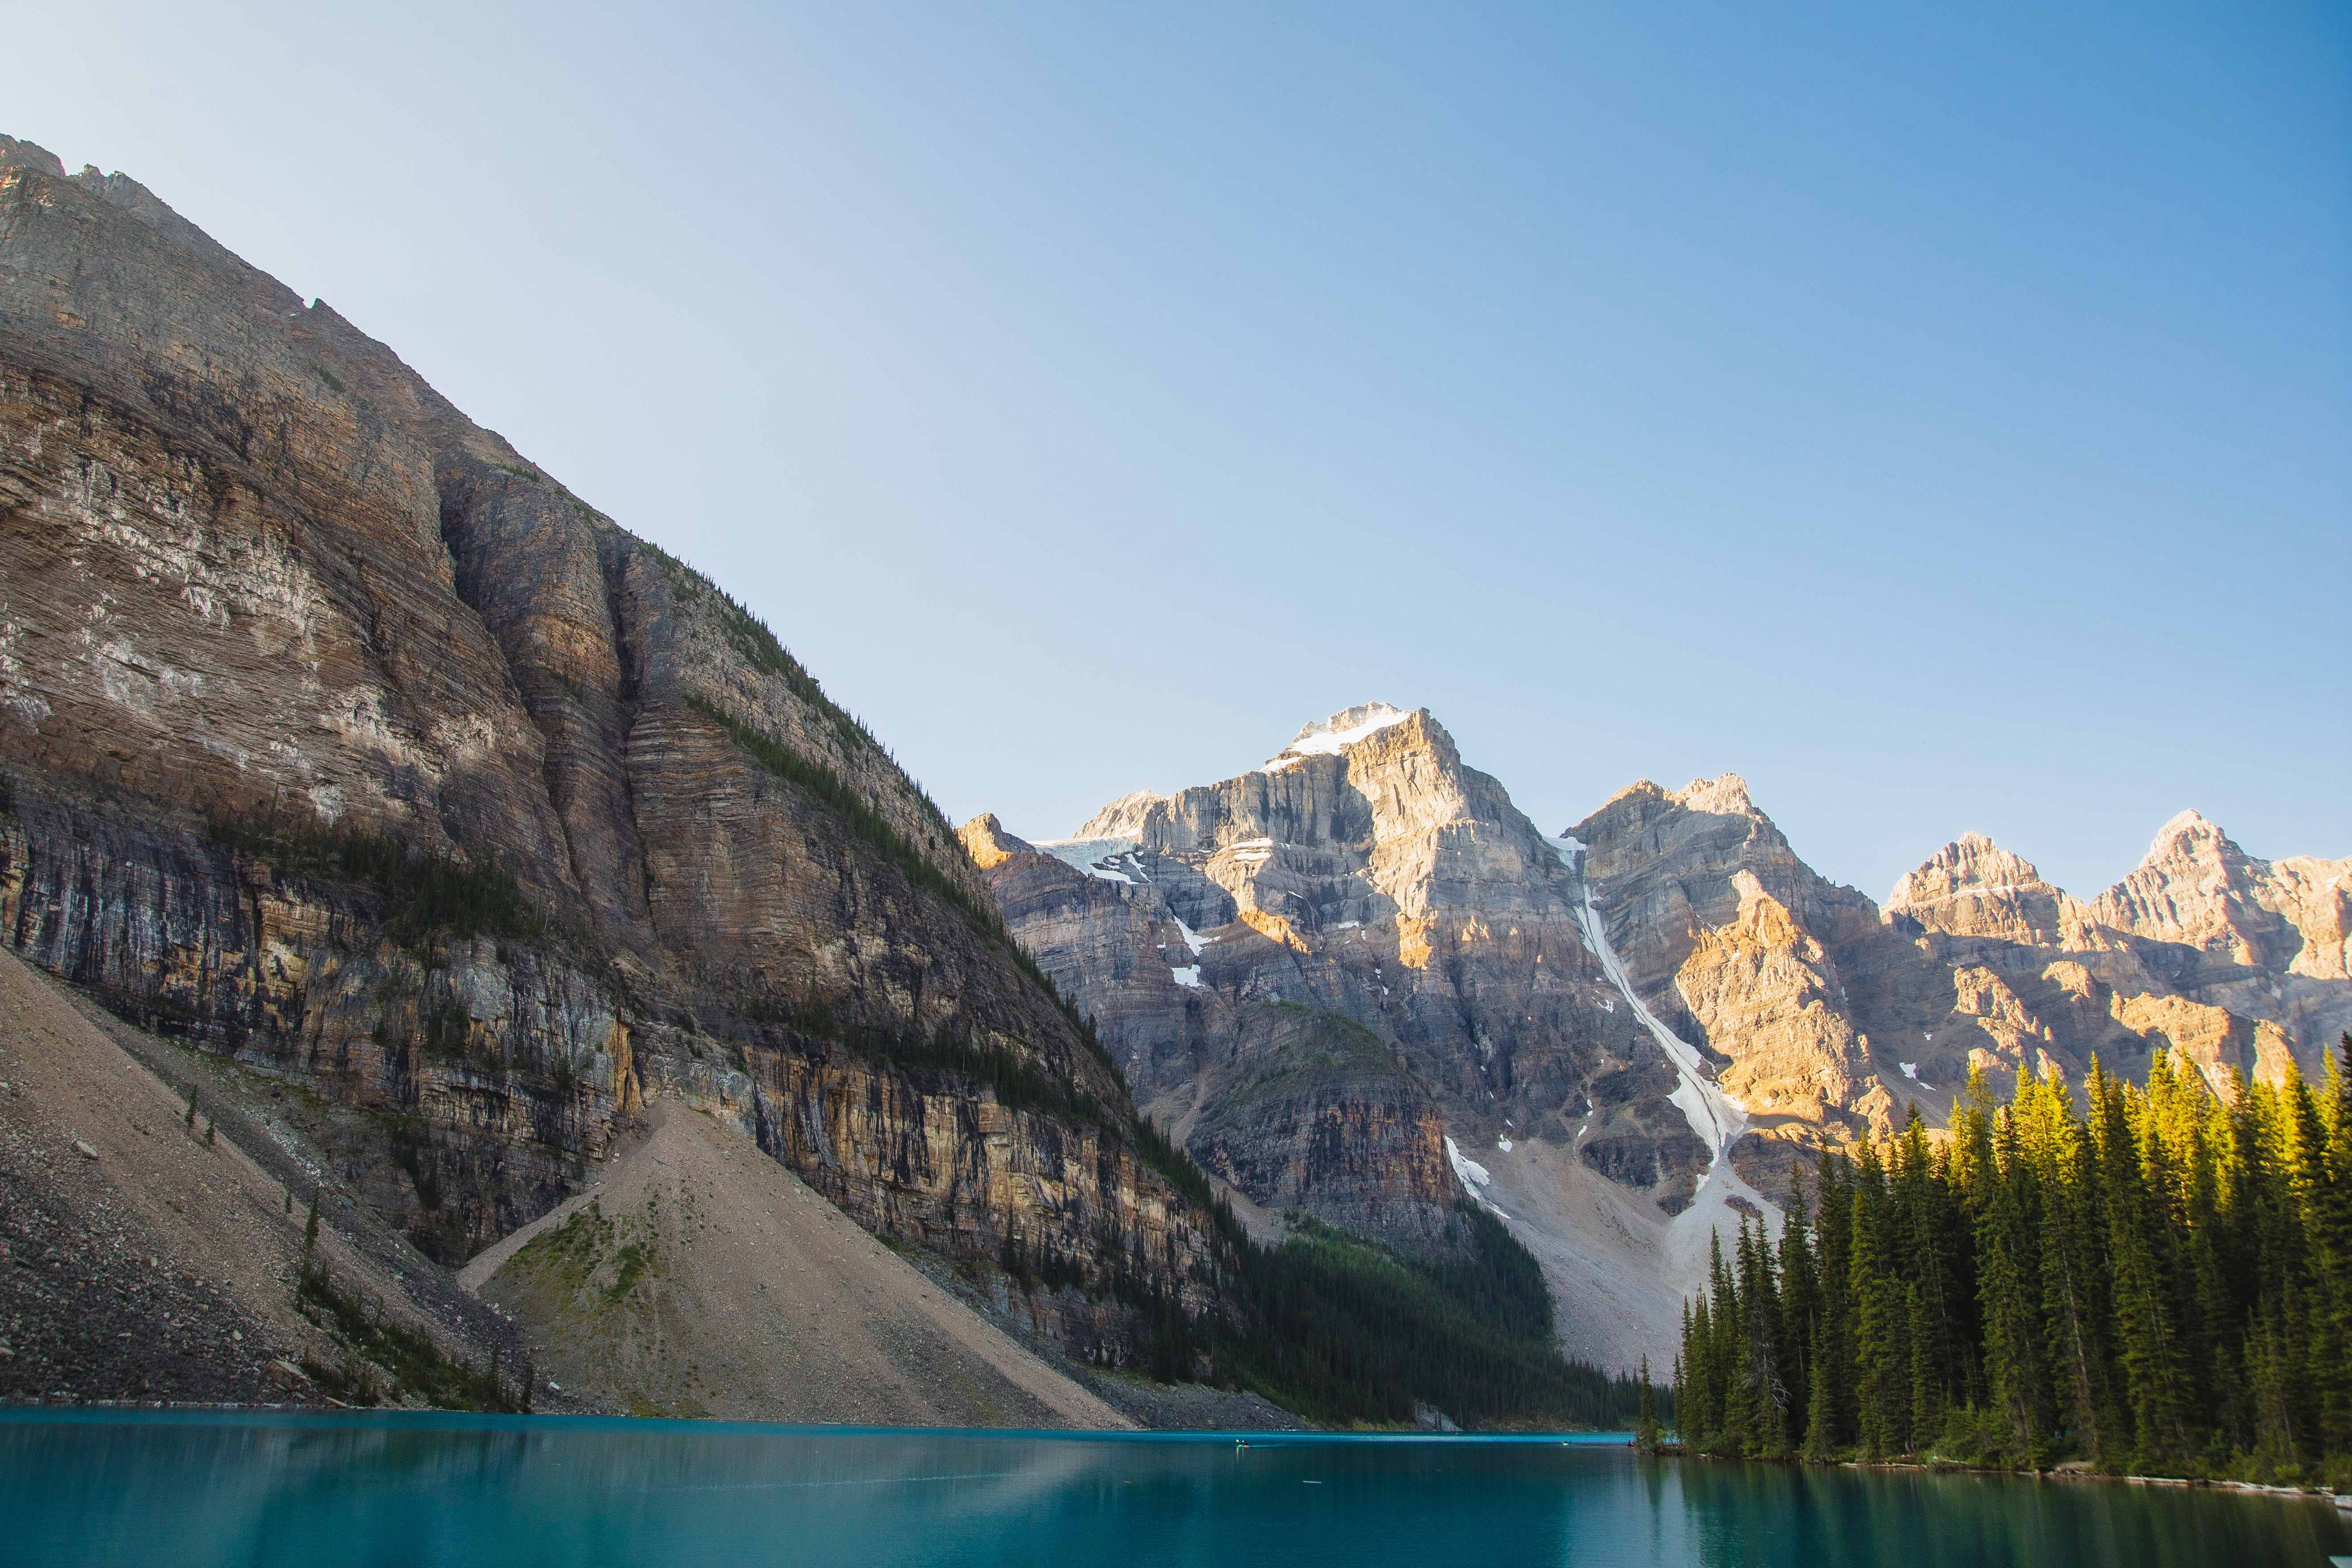
\includegraphics[angle=90,width=\textwidth]{img/mountain.jpg}
\end{flushleft}

\newpage
\section{Floating Bodies}
\verb|\begin{figure}[placement specifier] or \begin{table}[...]|

\subsection*{Float Placing Permissions}
\rule{0pt}{5ex}
\fbox{If no placement specifier is given, the standard classes assume [tbp].}\\
\rule{0pt}{2ex}

\begin{table}[!ht]
\caption{Float Placement Permissions}
{\renewcommand{\arraystretch}{1.5}
\begin{tabular}{c|l}
Specs           &       Permission                                                          \\
\hline
\texttt{h}      &       \parbox[t]{9.8cm}{%
Place the float \texttt{here}s,\\
i.e., approximately at the same point it occurs in the source text (however, not exactly at the spot)}  \\
\texttt{t}      &       Position at the \texttt{top} of the page.                                       \\
\texttt{b}      &       Position at the \texttt{bottom} of the page                                     \\
\texttt{p}      &       Put on a special \texttt{page} containing only floats only.                     \\
\texttt{!}      &       \parbox[t]{9.8cm}{%
Override internal parameters,\\
such as the maximum number of floats allowed on one page,\\
those \LaTeX{} uses for determinig ``good'' float positions.}                                           \\
\texttt{H}      &       \parbox[t]{9.8cm}{%
Places the float at precisely the location in the \LaTeX{} code.\\
Requires the float package (\texttt{\textbackslash{}usepackage\{float\}}).\\
This is somewhat equivalent to \texttt{h!}, though some errors may arise if you have too many consecutive floats with \texttt{[H]}.}
\end{tabular}}
\end{table}

\rule{0pt}{2ex}

\LaTeX{} will place every float it encounters according to the placement specifier supplied by the author.
If a float cannot be placed on the current page it is deferred either to the figures queue or the tables queue.15
When a new page is started, \LaTeX{} first checks if it is possible to fill a special 'float' page with floats from the queues.
If this is not possible, the first float on each queue is treated as if it had just occurred in the text:
\LaTeX{} tries again to place it according to its respective placement specifiers (except 'h,' which is no longer possible).
Any new floats occurring in the text get placed into the appropriate queues. \LaTeX{} strictly maintains the original order of appearance for each type of float.
That's why a figure that cannot be placed pushes all further figures to the end of the document. Therefore:

\begin{quote}
If \LaTeX{} is not placing the floats as you expected, it is often only one float jamming one of the two float queues.
\end{quote}

While it is possible to give \LaTeX{} single-location placement specifiers, this causes problems.
If the float does not fit in the location specified it becomes stuck,
blocking subsequent floats. In particular, you should never, ever use the \verb|[h]|
option—it is so bad that in more recent versions of \LaTeX{}, it is automatically replaced by \verb|[ht]|.

\newpage
\subsubsection{Captioning}

\rule{0pt}{2ex}

\fbox{\texttt{\textbackslash{}caption\{caption text\}}}

\rule{0pt}{2ex}

Defining a caption for the float.\\
A running number and the string ``Figure'' or ``Table'' will be added by \LaTeX{}.

\rule{0pt}{2ex}

For long captions:

\rule{0pt}{2ex}

\begin{figure}[!ht]
\fbox{\texttt{\textbackslash{}caption[short]\{loooooooooooooooooooong\}}}
\caption[Short]{Loooooooooooooooooooong (At the backmatter, on page: \pageref{tab:lsoffigs})}
\end{figure}

\rule{0pt}{2ex}

\fbox{\texttt{\textbackslash{}listoftables and \textbackslash{}listoffigures}}

\rule{0pt}{2ex}

These two commands operate analogously to the \verb|\tableofcontents| command.

\rule{0pt}{2ex}

Under certain circumstances it might be necessary to use either of these commands:

\rule{0pt}{2ex}

\fbox{\texttt{\textbackslash{}clearpage} or even the \texttt{\textbackslash{}cleardoublepage}}

\rule{0pt}{2ex}

It orders \LaTeX{} to immediately place all floats remaining in the queues and then start a new page. \texttt{\textbackslash{}cleardoublepage} even goes to a new right-hand page.

\newpage
Figure~\ref{white} is an example of Pop-Art.
\begin{figure}[!hbtp]
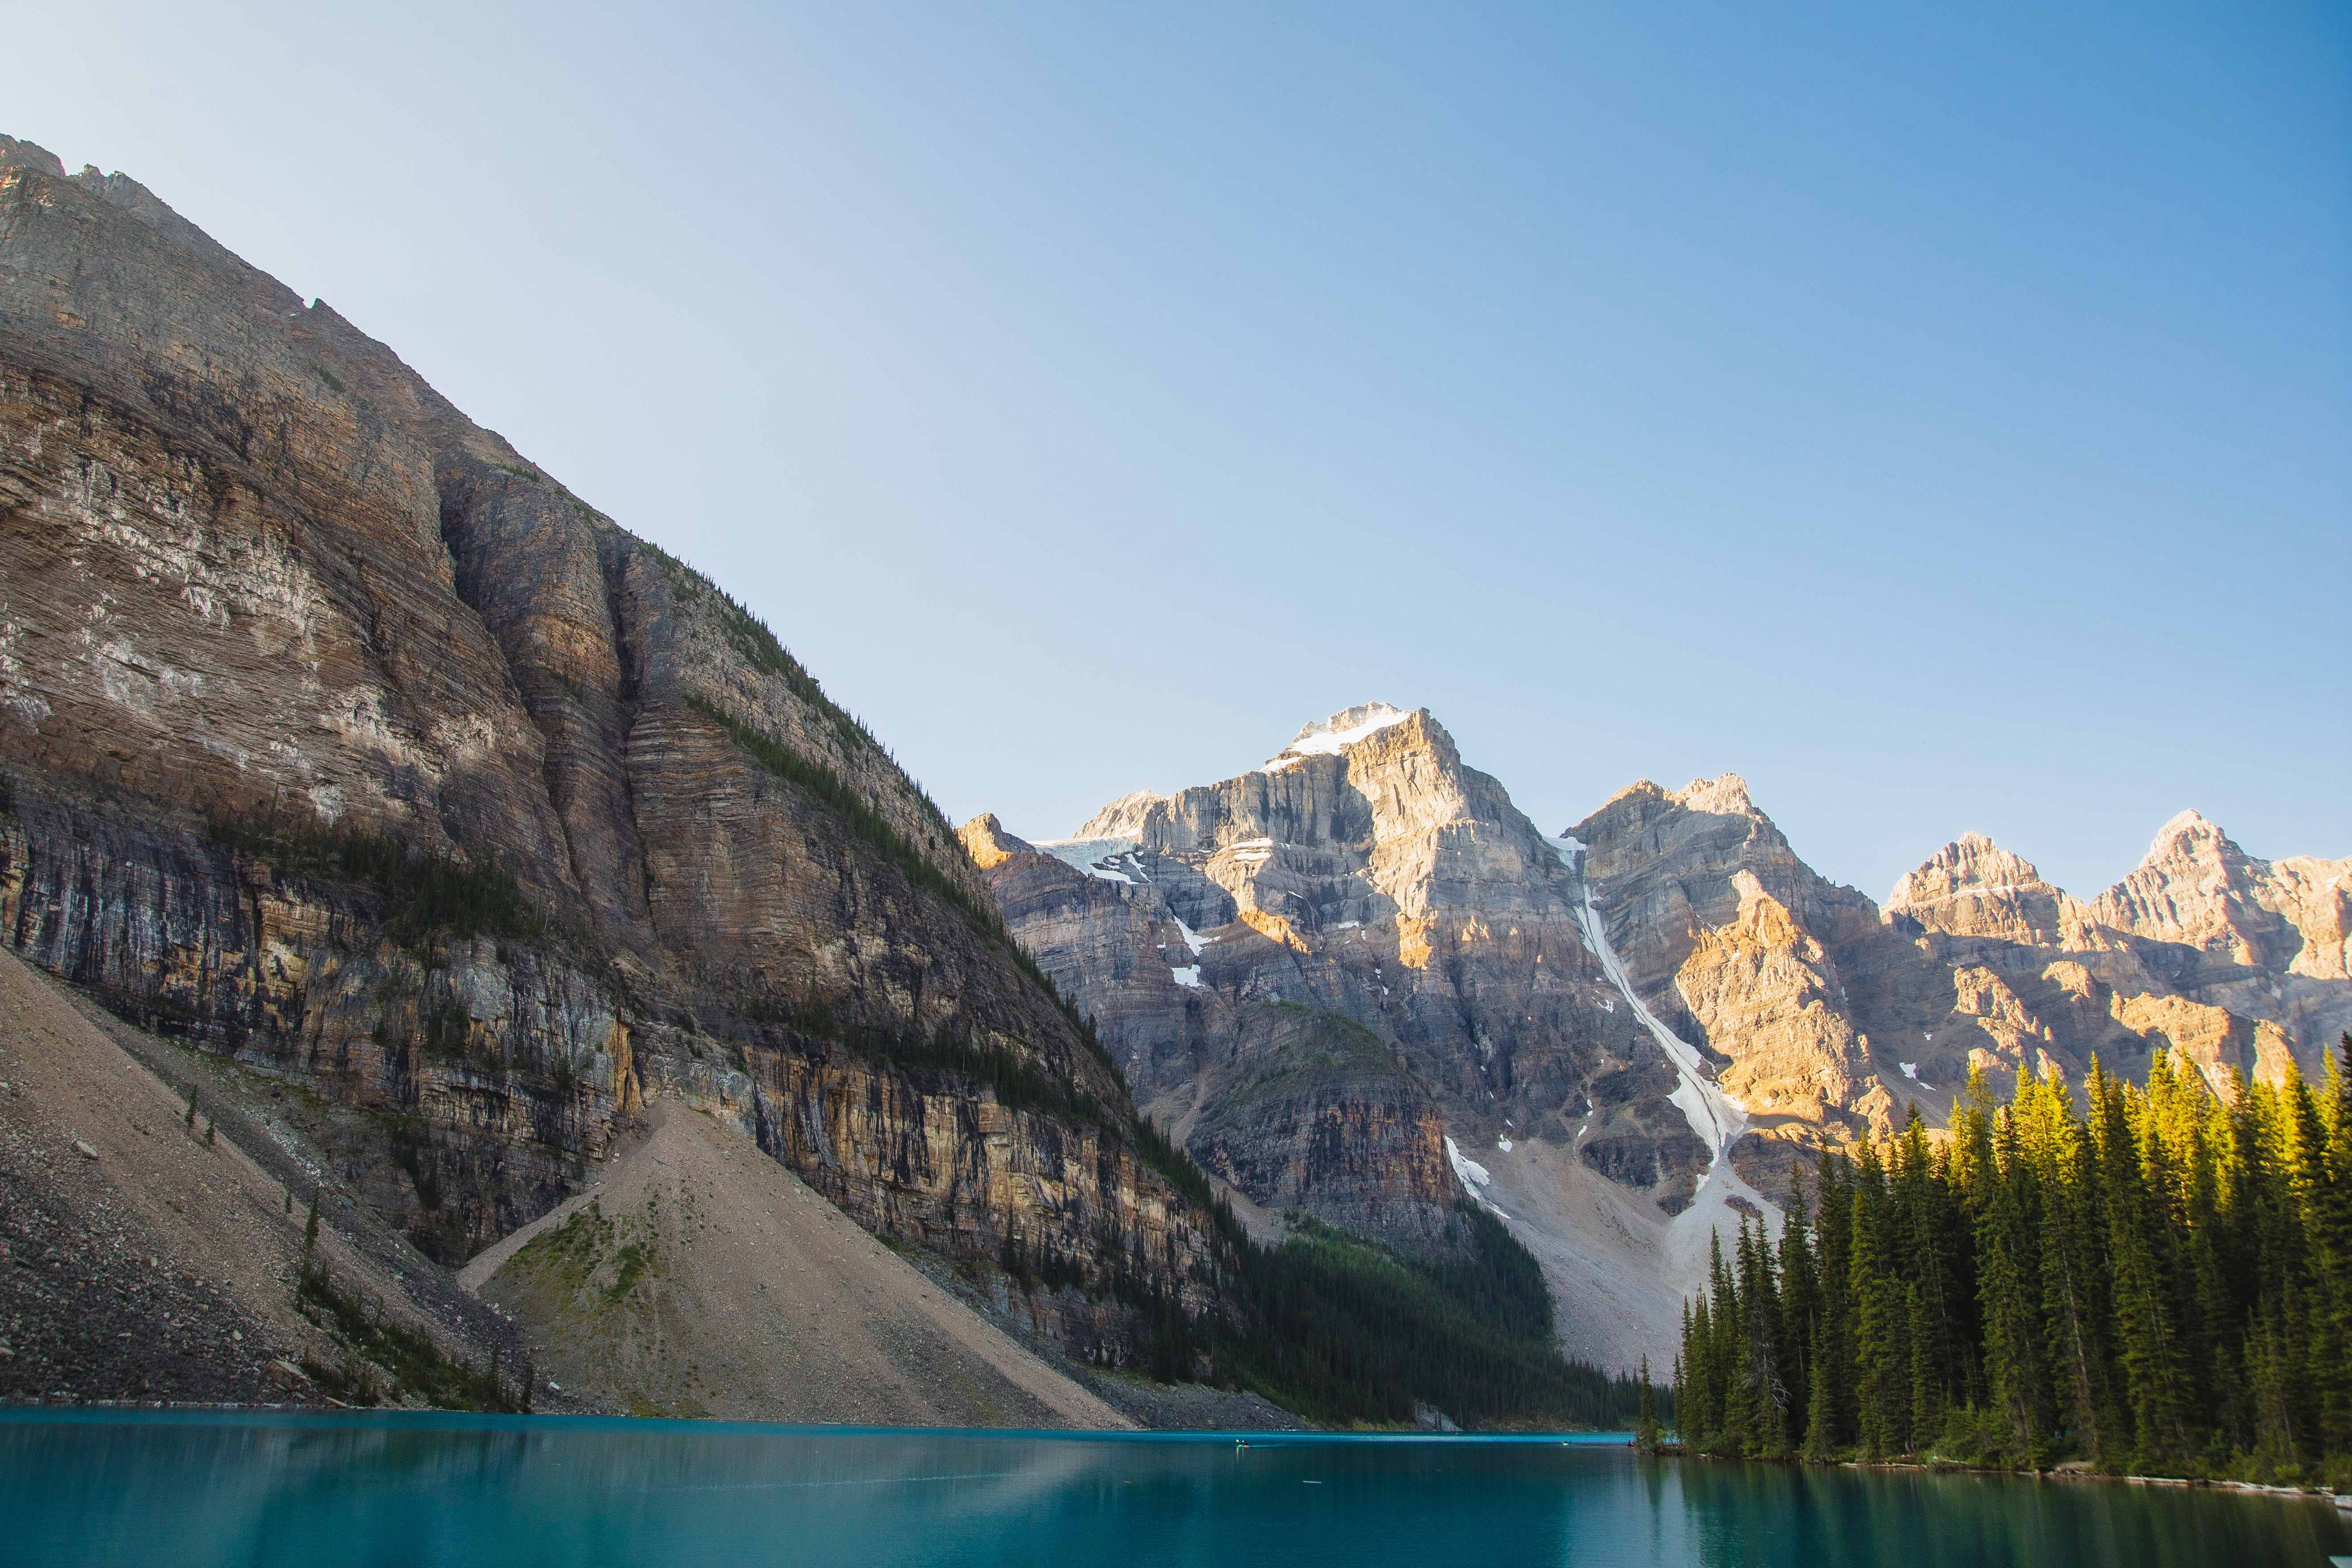
\includegraphics[width=\textwidth]{img/mountain.jpg}
\caption[Calm lake surrounded by mountains]{Calm lake surrounded by mountains by Ryutaro Tsukata.\label{white}}
\end{figure}

\newpage
\pagenumbering{roman}
\listoftables

\newpage
\listoffigures \label{tab:lsoffigs}
\end{document}